\newpage
\subsection{Design}
Designdiagrammet i projektets anden iteration, blev opdateret med flere klasser og en tydelig lagdeling. En klar adskillelse af præsentations-, domæne- og persistenslaget er blevet illustreret og indeholder også subsystemernes klasser, med attributter og metoder. Det er valgt at getter og setter metoder ikke vises i diagrammet, da det ville gøre det meget større og sværere at overskue. (Reference til bilaget, med det fulde designdiagram)\\
For at få et samlet overblik se interne bilag \ref{sec:diverse} figur \ref{fig:opklassemedlog} og figur \ref{fig:opklasse}\\
\textbf{Præsentationslaget}
\begin{figure}[htb!]
  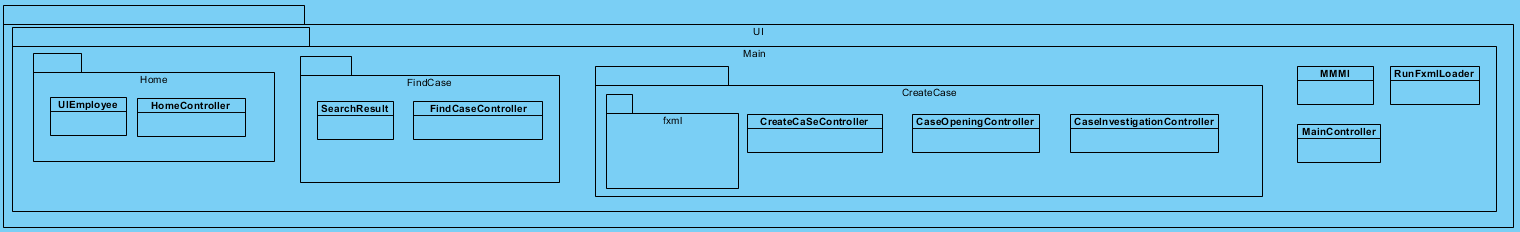
\includegraphics[width = \linewidth]{./PNG/design/UIopdateretKlassediagram.PNG} 
  \caption{Der blev valgt at undlade beskrivelsen af kontrollernes indhold og FXML-dokumenterne i subsystemet UI (Præsentationslaget), for at gøre diagrammet mere overskueligt. Præsentationslaget er blevet illustreret med pakker, som indeholder kontrollere og FXML-dokumenter for specifikke funktioner, samt klasserne som styrer systemets GUI.}
  \label{fig:2pre}
\end{figure}
\\\textbf{MMMI – Main Class}\\
Programmet køres gennem MMMI klassen, da det er programmets main class.\\
\textbf{MainController – Præsentations controlleren}\\
Klassen ”MainController”, er systemets primære FXML-handler. Den blev lavet så det var muligt at skifte funktionalitet, på baggrund af et brugerinput, i samme root-node.
\textbf{RunFxmlLoader – Præsentationsmetoden}\\
Klassen ”RunFxmlLoader”, indeholder funktionaliteten som bruges til at skifte FXML-dokumenter. Den bliver arvet af ”MainController”, og implementere, som det eneste, metoden der bruges til at skifte ”pane”, i systemet.\\
\textbf{CreateCase – Dokumentstyring og præsentation}\\
Subsystemet ”CreateCase”, blev designet til at begynde oprettelsen af nye sager i systemet og styre præsentationen af sagsdokumenter, samt brugerinteraktionen med disse. I slutningen af anden iteration var ”CreateCase”, pakket med kontrollerne ”CreateCaseController”, ”CaseOpeningController” og ”CaseInvestigationController”, samt FXML-pakken ”fxml”, som var pakket med de tilsvarende FXML-dokumenter.\\ 
Controlleren ”CreateCaseController”, blev designet til at styre bevægelsen mellem sagsdokumenter, samt at gemme brugerindtastet information fra disse dokumenter. Navngivningen kunne virke misvisende, i forhold til at controlleren bruges til at skifte mellem dokumenter, men peger på funktionaliteten bag gem funktionen. Når en given bruger benytter gem funktionen i en sag, sender controlleren de brugerindtastede informationer til domænelaget, for at få det registreret i systemdatabasen. \\
Hvis en sag gemmes for første gang i systemet, vil informationen som sendes gennem systemlagene, oprette en ny sag i databasen, som derefter modtager informationen. Controlleren er blevet navngivet efter denne proces, men har i sig selv kun at gøre med brugerinput og kommunikationen med domænelaget.\\
Controlleren ”CaseOpeningController”, er designet til at pakke informationerne indtastet i FXML-dokumentet ”caseOpeningNew”, og derefter sende det videre til ”CreateCaseController”, når en given bruger benytter gem funktionen.\\
Controlleren ”CaseInvestigationController”, har at gøre med informationen fra FXML-dokumentet ”caseInvestigation”. Controlleren er designet ligesom ”CaseOpeningController”, da de begge er designet til at håndtere information fra FXML-dokumenter, som er designet efter dokumenterne fra VUM. (kilde) \\
Designet af ”CreateCase”, var planlagt med fremtidig udvikling i tankerne, for at lave og implementere de dokumenter fra VUM, som mangler.\\
\textbf{FindCase – Sagsrelateret søgning} \\
Subsystemet ”FindCase”, er designet til at håndtere et brugerinput, i form af en søgning, og præsentere information relateret til søgeordet. Subsystemet består af klassen ”SearchResult” og controlleren ”FindCaseController”, samt FXML-dokumentet ”findCase”.\\
Klassen ”SearchResult”, er en placeholder som fyldes med den data, der hentes på baggrund af en given brugers søgeord. Controlleren ”FindCaseController”, henter informationen som ”SearchResult”, består af og præsentere dem gennem FXML-dokumentet ”findCase”.\\
\textbf{Home – Systemets startside} \\
Subsystemet ”Home”, er designet til at håndtere systemets startside. Subsystemet består af klassen ”UIEmployee”, som er en placeholder klasse for medarbejderen der er logget ind i systemet og controlleren ”HomeController”, samt FXML-dokumentet ”home”.\\
Klassen ”UIEmployee”, er en placeholder klasse, som fyldes med information relateret til medarbejderen der er logget ind i systemet. Controllerklassen ”HomeController”, bruger informationen fra ”UIEmployee”, til at finde de relevante informationer som vedrør medarbejderen og præsentere dem gennem ”home”-dokumentet.\\
\textbf{Domænelaget}
\begin{figure}[htb!]
  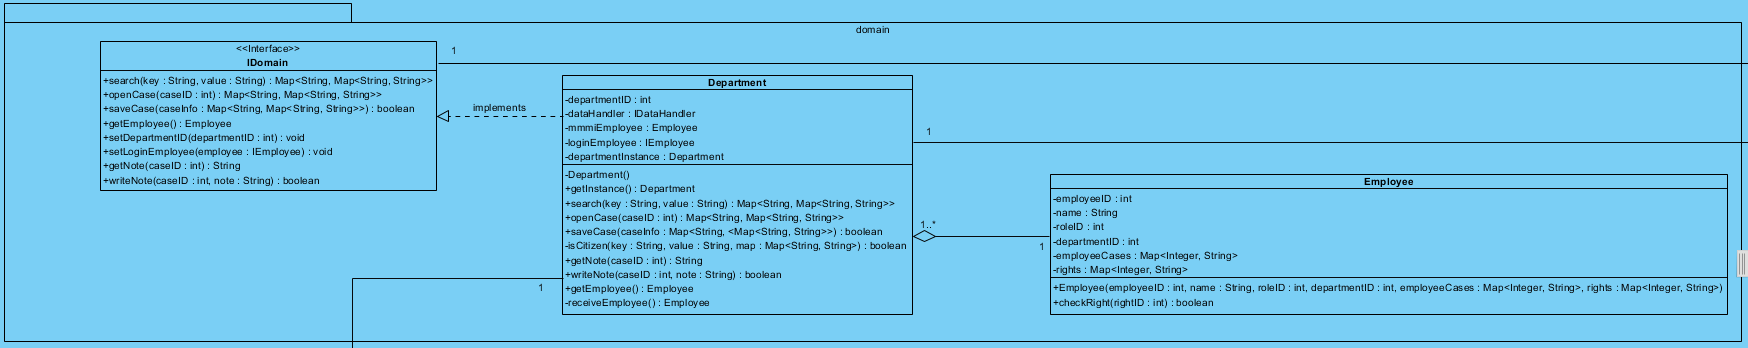
\includegraphics[width = \linewidth]{./PNG/design/domaeneOpdateretKlassediagram.PNG} 
  \caption{Domænelaget er blevet designet med to klasser, med attributter og metoder, og et interface.}
  \label{fig:2dom}
\end{figure}
\\\textbf{IDomain – Provided interface}\\
IDomain interfacet bruges til at vise præsentationslaget hvilke metoder der er tilgængelige i domænelaget, hvad de returnerer samt hvilke attributter der er nødvendige for at benytte metoderne. Interfacets metoder bliver implementeret i ”Department” klassen.\\
\textbf{Department – Facadeklasse}\\
Klassen ”Department” har en private constructor “Department()”, attributterne ”departmentID”, ”dataHandler”, ”mmmiEmployee”, ”loginEmployee” og ”departmentInstance”, samt metoderne ”getInstance()”, ”search(…)”, ”openCase(…)”, ”saveCase(…)”, ”isCitizen(…)”, ”getNote(…)”, ”writeNote(…)”, “getEmployee()” og “receiveEmployee()”.\\
For at imødekomme projektets underspørgsmål ”Hvordan sikres det at aktøren kun har adgang til det aktøren har brug for?” og dataafgrænsningen fra sagsudredning i semestercasen, er der blevet lagt stor vægt på attributten “departmentID”. \\
Dette ID tildeles via en setter metode, ”setDepartmentID(…)”, når en medarbejder logger ind i systemet. Singleton designpattern blev valgt, da der er nødvendigt at være sikre på at det er det samme ”Department”-objekt der arbejdes med gennem hele systemet.\\
\textbf{Employee – Dataklasse, repræsenterer den medarbejder der er logget ind}\\
Klassen ”Employee” er designet til at håndtere tjek af rettigheder i forhold til forskellige medarbejderroller. Når en bruger logger ind i systemet, sendes der en employeeID til ”Department” som kalder persistenslaget for at få data om medarbejderen for at oprette en instans af Employee.\\
Dette gøres for at det kan være muligt at der er styr på hvem der er logget ind, samt have mulighed for at tjekke rettighederne som medarbejderen har gennem metoden ”checkRight(…)”.\\
\textbf{Persistenslaget}
\begin{figure}[htb!]
  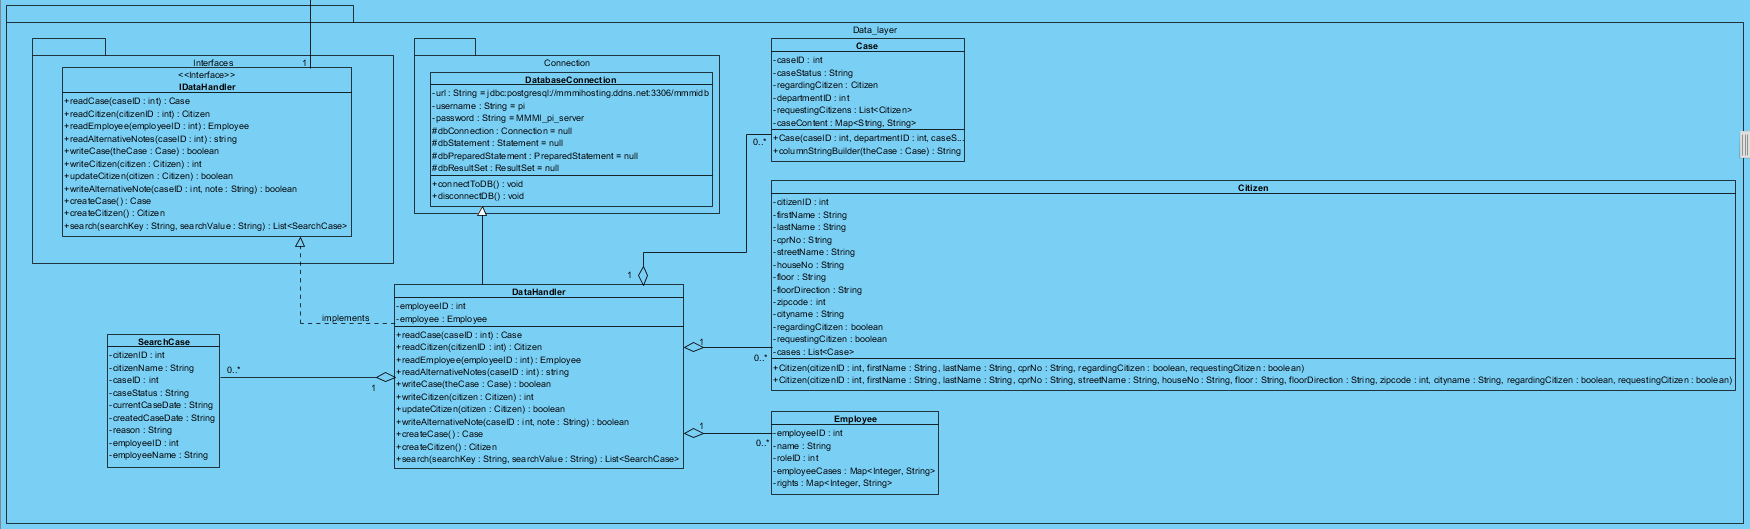
\includegraphics[width = \linewidth]{./PNG/design/datalagKlassediagram.PNG} 
  \caption{Persistenslaget er blevet designet med seks klasser og et interface.}
  \label{fig:2dataklassediagram}
\end{figure}
\\ 
\textbf{IDataHandler – Provided interface} \\
Interfacet ”IDataHandler”, bruges til at tillade og etablere kontakten mellem domænelaget og persistenslaget. Metoderne som interfacet består af implementeres i ”DataHandler” klassen og kaldes i domænelaget, når databasen skal kontaktes.\\
\textbf{DataHandler – Facadeklasse}\\
Klassen ”DataHandler”, er blevet designet til at håndtere dataforespørgsler sendt fra domænelaget og behandle dem som ønsket i systemets database. Klassen implementerer ”IDataHandler” interfacet og metoderne der følger med, som specificeres så data bliver hentet og/eller gemt, når de bliver kaldt fra domænet.\\
Når der skal hentes data fra databasen, er metoderne ”readCase(…)”, ”readCitizen(...)”, ”readEmployee(…)”, ”readAlternativeNotes(…)” og ”search(…)”, blevet designet for at kunne tilgå specifikke koloner, så den relevante information kan blive hentet. \\
Designet er lavet så at, når der skal gemmes data i databasen, benyttes metoderne ”writeCase(…)”, ”writeCitizen(…)”, ”updateCitizen(…)” og ”writeAlternaticeNote(…)”. Metodekaldet der skal bruges, afhænger af hvilken information der ønskes gemt. \\
Klassens associationer består primært af aggregeringer, med multipliciteten one-to-zero-or-many. ”DataHandler” er forbundet med aggregeringer til klasserne ”SearchCase”, ”Case”, ”Citizen” og ”Employee”. \\
\textbf{SearchCase – Placeholder til data fra “search(…)”}\\
Klassen ”SearchCase” indeholder udelukkende attributterne ”citizenID”, ”citizenName”, ”caseID”, ”caseStatus”, ”currentCaseDate”, ”createdDateCase”, “reason”, “employeeID”, “employeeName”.  Klassen bruges når der søges i databasen med metoden ”search(…)”, til at indeholde de data der er relevant at vise brugeren, i forhold til at kunne vælge den rigtige sag at åbne.\\
\textbf{Employee – Dataklasse, repræsenterer en medarbejder og alle dennes tilknyttede sager i afdeling}\\
Klassen ”Employee” indeholder udelukkende attributterne ”employeeID”, ”name”, ”roleID”, ”employeeCases” og ”rights”. \\
\textbf{Case – Dataklasse, repræsenterer en sag}\\
Klassen ”Case” indeholder attributterne “caseID”, “caseStatus”, “regardingCitizen”, “departmentID” som alle skal bruges for at oprette en ny sag i tabellen ”case” i databasen. Yderligere er der en attribut ”requestingCitizen”, som skal bruges for at forbinde en sag med en eventuel henvendende borger, samt en attribut ”caseContent”, som indeholder alle oplysninger som en sagsbehandler kan indtaste. \\
Der er også en constructor som sætter alle attributterne, samt en metode der bruges til at konstruere den query, som sørger for at ”caseContent”, bliver gemt i databasen.\\
\textbf{Citizen – Dataklasse, repræsenterer en borger og alle dennes oprettede sager i afdeling}\\
Klassen ”Citizen” indeholder attributterne ”citizenID”, ”firstName”, ”lastName”, ”cprNo”, ”streetName”, ”houseNo”, ”floor”, ”floorDirection”, ”regardingCitizen”, ”requestingCitizen”, ”Cases”. Den har 2 constructore, en som har de primære attributter der skal bruges for at oprette en Citizen i database, og en anden som har alle attributter.\\
\textbf{DataConnection – Håndtering af forbindelse til database}\\
Klassen ”DataConnection” blev implementeret for at vi kunne have de nødvendige informationer til at forbinde med databasen placeret et sted som kunne genbruges i andre moduler. \\
\subsubsection{Dynamisk design}
\textbf{Search}
Når en sagsbehandler eller leder skal søge igennem databasen for at finde en specifik sag. \\
I det en aktør klikker på søg knappen, bliver der lavet en efterspørgsels ud fra en specifik søge nøgle i form af String send fra presistenslageret til Departpartment i domainlageret. Denne string bliver sendt til Datahandleren. Hvor metoderne search bebrejder stringen efter om det er en borger eller en case der søges på. Afhængig af hvilken form af søgn, vil der blive sende en anmodning til database, hvor da validere om den specifikke søgning eksister. Vis den eksister sender databasen et resultset tilbage med de informationer der er ud fra den specifikke case. Den data bliver omdannes til nye objekter af ScearchCase.\\
disse objecter lægges i en liste af objecter SceartchCase. Herefter bliver det send tilbage til Department, Hvor dataene bliver delt op i forskellige Kategorier og lægges i et map ”ResultsetMap”. ResultsetMap sende er efter op til UI. I UI bliver ResultsetMap omdannet til objectet SearchResultset. Som bliver vis til aktøren. \\
Search er bygget efter aktøren behov for at finde en specifik sag på en borger. Hvor der skal være mulighed for at ændre eller vider bygge på en sag om en borgen. \\
VI har valgt at lader datalageret håndtere ansvaret for validere søgningen eftersom det er den der er den stærkeste tilknytning til databasen og for at reducere den gennerale kobling i projektet, hvilket der er lagt meget Vægt på i projektet.\\
\textbf{saveCase}
Når en aktør ar udfyldt noget af sagsoplysningerne i en sag. Har aktøren muligheden for at gemme arbejdet i databasen ved at klikke på gem. \\
Når en aktør klikker på gem sendes der et Map af strings ned fra presistenslageret til Departpartment.\\
I Department bliver der valideret om sagsindholdet. Map kan indeholde et caseID der er ligmed -1. vis dette er tilfældet vil der blive kaldt metode CreateCase i IDatahandler. Methodes formål er at lave et nyt object af Case med den information der er givet, herefter sendes tilbage til Department. \\
Vis caseID ikke er -1 vil er ikke blive lavet et nyt objekt. Da dataene ligger i et eksisterer objekt af case Her vil updateCase bliver kaldt. Updatecase’s formål er at opdatere objektet med den information der er giver. \\
Department sender nu ned til Datahandleren gennem interfaceset IDatahandler ved brugen af metoden WriteCase. WriteCase valider igen om caseID = -1. vis det er -1 vil der laves en peparesStatment der sender casens data til databasen. Og den sender en true op igennem systemet.
